\appendix

\section{Appendix}


\subsection{Algorithm Properties}
\label{sec:proof}

%\todo{Dan will fill this in.}
%The reason why this work is our high-level design and the distributed share calculation. The distributed share calculation makes sure that the starting allocation is feasible. This allows us to do packing based on free channels. If the initial share wasn't feasible, the algorithm would have issues converging (Dan has a proof for this). This is why the packing idea is fundamentally suitable for our approach.

We now analyze the properties of the assignment framework given in ~\ref{sec:channel-selection}. 
In particular, we will give a sufficient condition under which the basic hopping algorithm 
(without the channel re-use heuristic) is guaranteed to converge, 
and probabilistic convergence bounds in this case. 

More precisely, we abstract the given setting as an undirected graph $G = (V, E)$, where each vertex $v_i \in V$ corresponds to an \eNB $i$. 
Further, two vertices $v_i$ and $v_j$ are connected by an edge if $v_i$ may interfere with one of $v_j$'s clients, or vice-versa. 
Let $N(v_i)$ denote the graph neighborhood of node $v_i$. 
Vertices share a set of $M$ subchannels, and initially each vertex $v_i$ has integer demand $d_i \geq 0$, which corresponds to the sum of user shares computed by the algorithm. 
Our analysis makes the assumption that, in every neighborhood, there exists a constant factor difference between the sum of demands and the total number of  subchannels.

\begin{eqnarray*}
  \textnormal{There exists a constant } 1 / M < \gamma \leq 1, \textnormal{ such that: } \\ \textnormal{ for every node }  v_i, \sum_{\ell \in N(v_i)} d_\ell \leq (1 - \gamma) M.
\end{eqnarray*}

Further, our analysis models subchannel fading by admitting a probability $0 \leq p < 1$ that a subchannel sensed as \emph{free} (and therefore chosen by the hopping procedure) is in fact unusable by the node. 
This failure event is assumed to be independent of the nodes' random hopping choices, and across hopping rounds. 

We focus on \emph{convergence time}, i.e., the time required for the algorithm to reach a configuration in which each node has its subchannel demand fulfilled, and stops hopping. 
We prove the following. 

\begin{thm}
\label{thm:convergence}
	Under the above assumptions, the algorithm is guaranteed to converge with probability $1$. The algorithm will converge in $O( M \log n / ((1 - p) \cdot \gamma) )$ rounds, both in expectation and with high probability.   
\end{thm}
\begin{proof}
	Let us consider the process by which a node $v$ satisfies a unit of its demand. By assumption, the following hold: 1) the node $v$ will not hop on a subchannel currently occupied by another node $v'$ and 2) since a node $v_\ell$ may only occupy $d_\ell$ subchannels in a round, and $\sum_{\ell \in N(v)} d_\ell \leq (1 - \gamma) M$, there exist at least $\gamma M \geq 1$ subchannels which are available at every hopping attempt. Therefore, given a hopping attempt by $v$, there are two conditions under which it does not succeed in acquiring the channel: either another node makes the same choice, or the channel is faded. These events occur independently, and, by assumption, the probability that node $v$ satisfies one unit of demand in a hopping attempt is at least $(1 - p) \gamma$.  
	
	Since round choices and fading are assumed to be independent across rounds, the expected time for the fixed node to satisfy a unit of demand is $ 1 / (\gamma (1 - p))$. By a Chernoff bound, for any constant $k \geq 2$, there exists a constant $c \geq 1$ such that the probability that the node fails to satisfy a unit after $k \log n / (\gamma (1 - p) )$ consecutive hopping attempts is at most $1 / n^c$. 
	By a union bound on the number of nodes, the probability that there exists \emph{some} node which fails after $k \log n / (\gamma (1 - p ))$ consecutive hopping attempts, is at most $1 / n^{c - 1}$. 
	The claim then follows by noticing that a node's demand is of at most $M$ subchannels. 
\end{proof}


It is interesting to consider the effect of channel packing on convergence. 
Technically, a larger channel slack $\gamma$ may be needed if hopping and packing occur concurrently, as packing may increase collisions. 
However, the fact that packing occurs after the node stops hopping ensures that the two procedures are independent to some degree.
The empirical evaluation confirms that convergence still occurs with packing, even for dynamic traffic patterns. 




%If  $Share_{ij}$ was decreased from this phase is lesser than the previous phase the eNB picks new sub-channels equal to the difference based on the reported CQI from $client_j$, if its greater eNB picks the best sub-channels from the ones previously assigned to $client_i$ that satisfy the new share.

%% \subsubsection{Implementation Details}
%% \label{other}

%% \noindent We now specify some key  implementation details. 


%% \noindent {\bf Channel Packing:} 
%% A useful optimization is the efficient packing of clients to channels, to enable spatial reuse. 
%% For example, clients which are very close to their respective base-stations are not likely to interfere with each other, and hence it would be beneficial for them to get the same allocation. 
%% While this is difficult to achieve without additional coordination, our design uses the following heuristic: 
%% each client maintains a leaky bucket corresponding to each channel it is assigned to. 
%% The client will move to a channel \emph{of lower index} if this channel is detected as \emph{free} for a certain contiguous period of time. 
%% The idea is that clients which experience low interference (such as the ones close to the base-station), will gradually move towards lower-index channels, and spontaneously self-organise. Moreover, as observed on the test topologies, convergence is reasonably fast. 




%% \noindent {\bf Scheduling:} Resources are allocated to an access point using the algorithm above. However, they are not strictly assigned to any specific client. Each access point can schedule any of its clients into any of the resource blocks it has acquired using any local scheduling algorithm. In our evaluation, we use the standard proportionally fair scheduling algorithm to schedule clients in order to achieve fairness across clients and combat channel selectivity. 

%% \noindent {\bf Detecting remaining interference: } As discussed in Section~\ref{issues}, an access point may incorrectly compute its share and take too many resources, due to sensing asymmetry. 
%% More precisely, the \eNB may believe that some resources are available, even though other access point potentially interferes on these resource blocks at the corresponding client. This type of interference is detected through client's CQI reports. If an \eNB observes a significant drop in the CQI for one or more resource blocks, the access point decides that the corresponding resource blocks are busy and removes them from the allocation.

%% \noindent {\bf Fairness in Cell-Fi:} There are several ways to define fairness in our context. We use temporal fairness for two reasons. The first is that it gives each user a the same time to access the spectrum, i.e. the shared resource. 
%% The second reason is that we can easily estimate the number of users, but not much else. Hence, any kind of proportional fairness based on rates is impossible, since we do not have any estimate of the rate. 

%% \todo{DAN: I think this discussion should be moved after the evaluation.} 
%% In our evaluation, we note that Cell-Fi tends to allocate more resources to remote nodes, when compared to other schedulers such as Fermi~\cite{fermi}. This reflects our choices of using low frequencies and focusing on coverage. 
%% Nodes which are closer to the \eNB can use higher frequencies to achieve connectivity. 


\begin{figure}[htb!]
  %\hfill
  %\begin{minipage}{0.33\textwidth}
  %  \centering
  %  (a)
  %  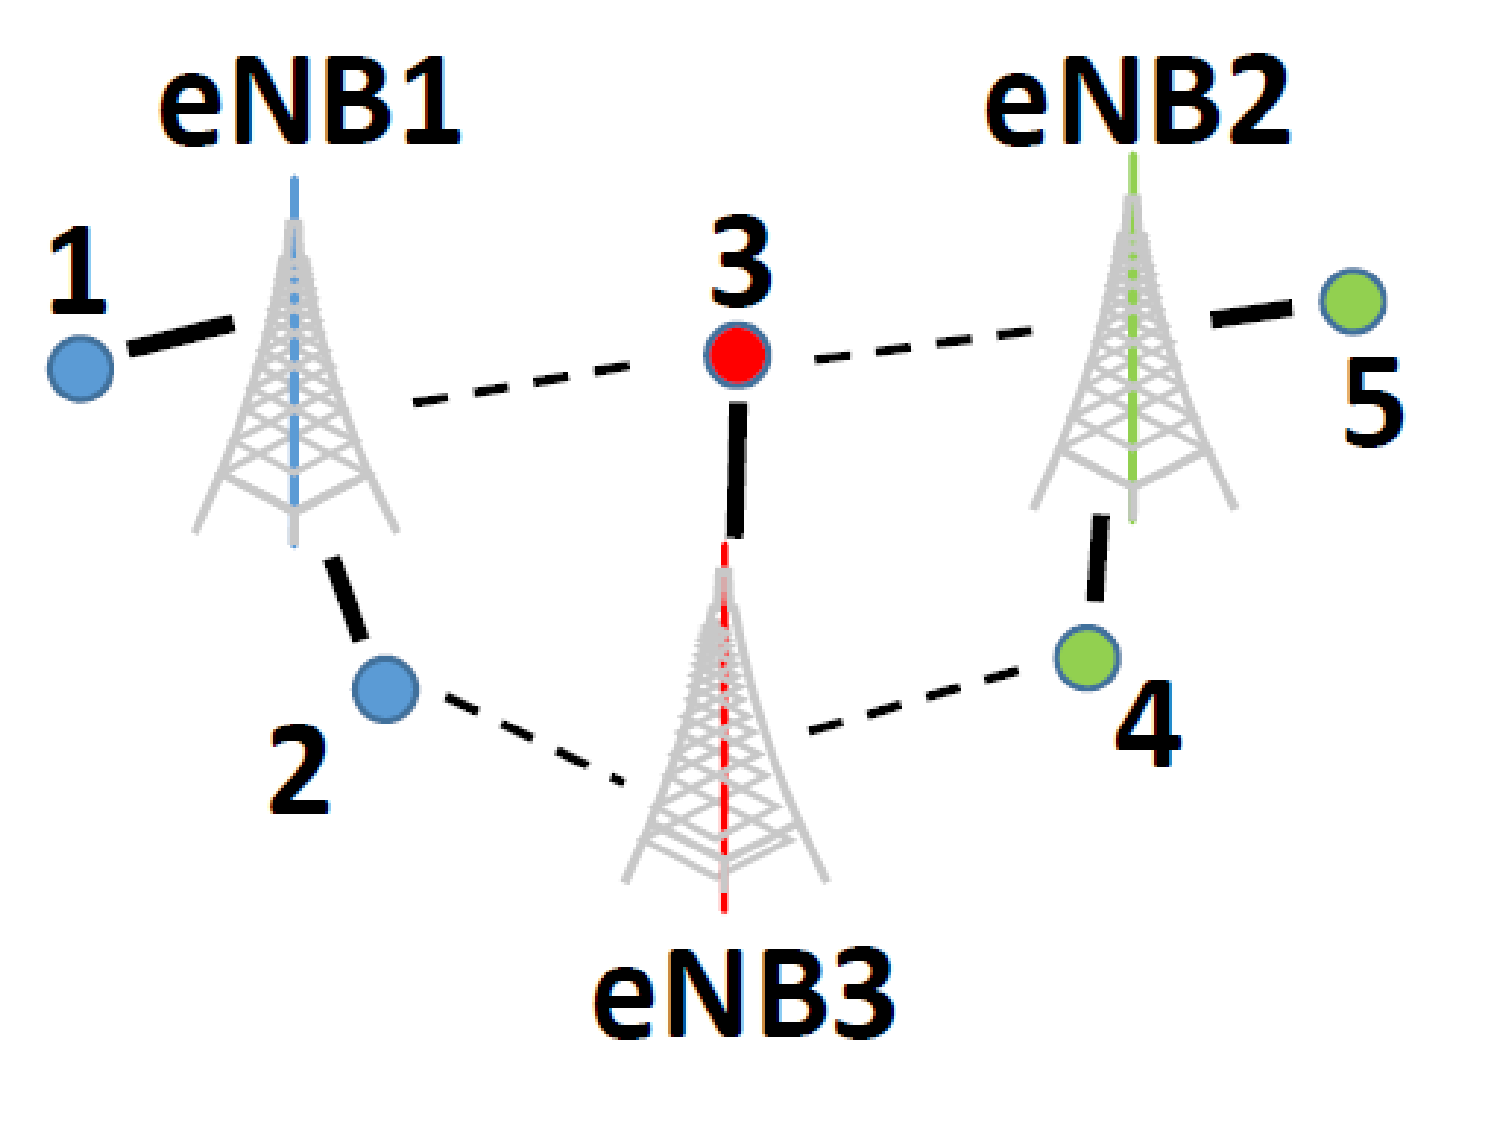
\includegraphics[width=\textwidth,height=0.6\columnwidth]{./figs/pack.pdf}
  %\end{minipage}
  %\hspace{1pt}
  \begin{minipage}{0.23\textwidth}
    \centering
    (a)
    \vfill
    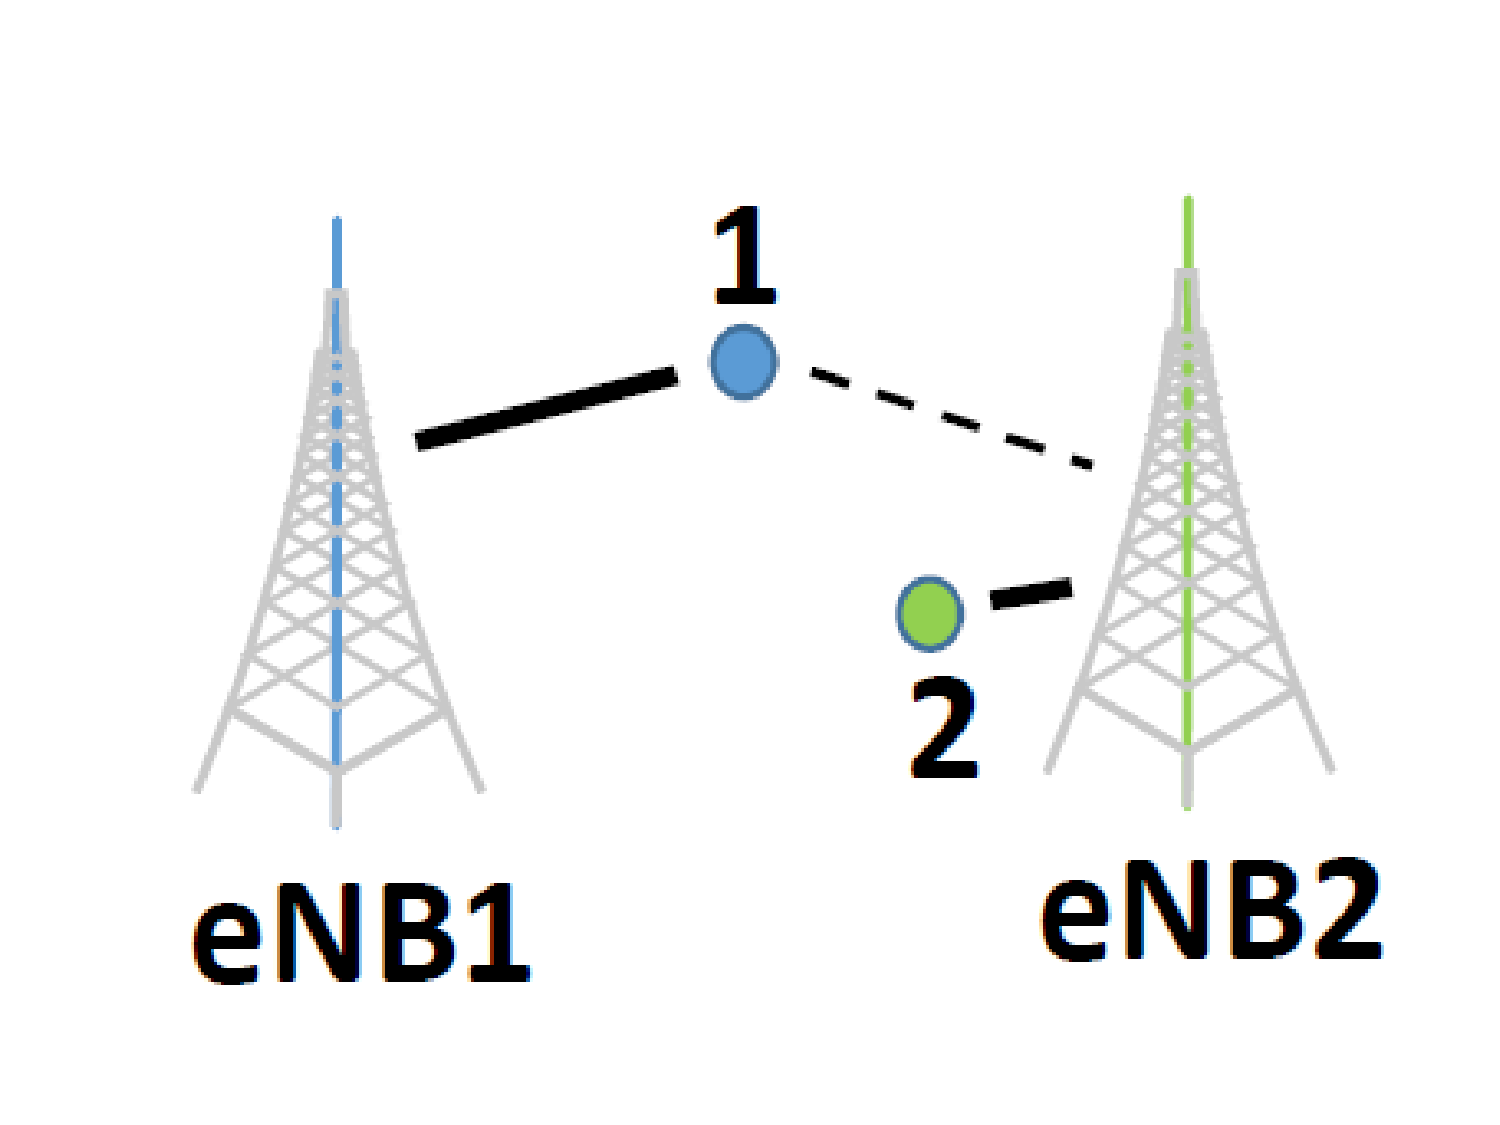
\includegraphics[width=\textwidth,height=0.6\columnwidth]{./figs/over.pdf}
  \end{minipage}
  \begin{minipage}{0.23\textwidth}
    \centering
    (b)
    \vfill
  \includegraphics[width=\textwidth,height=0.6\columnwidth]{./figs/under.pdf}
  \end{minipage}
  \hfill
  \caption{Lines reflect associated clients to access points while dashed lines reflect interference. }
%(a) Importance of channel re-use. client 3 can only get its share if access points 1-2 schedule their clients on same two channels. 
%(a) Information asymmetry with two total channels. access point 1 overestimates his share because it cannot sense client 2. (b) Informatrion assymetry with 4 total channels. 
%access point 2 has a share of 1, and while access point 1 can increase his share to 3, 
%it only reserves his fair-share, i.e., 2 channels because it does know how many subchannels 2 is using (1 due to clients 3-5)}
  \label{fig:asym}
\end{figure}


\subsection{Effects of information asymmetry}
\label{sec:asymmetry}


Wireless sensing depends on node location, and different nodes will obtain different views of the network. 
Every distributed wireless coordination protocol has to deal with this information asymmetry. 
The best known examples of information asymmetries in WiFi are exposed and hidden terminals. 
The distributed share calculation algorithm of \cf also suffers from two cases of information asymmetry, 
described below. 





%\begin{figure*}[t]
% \centering
%    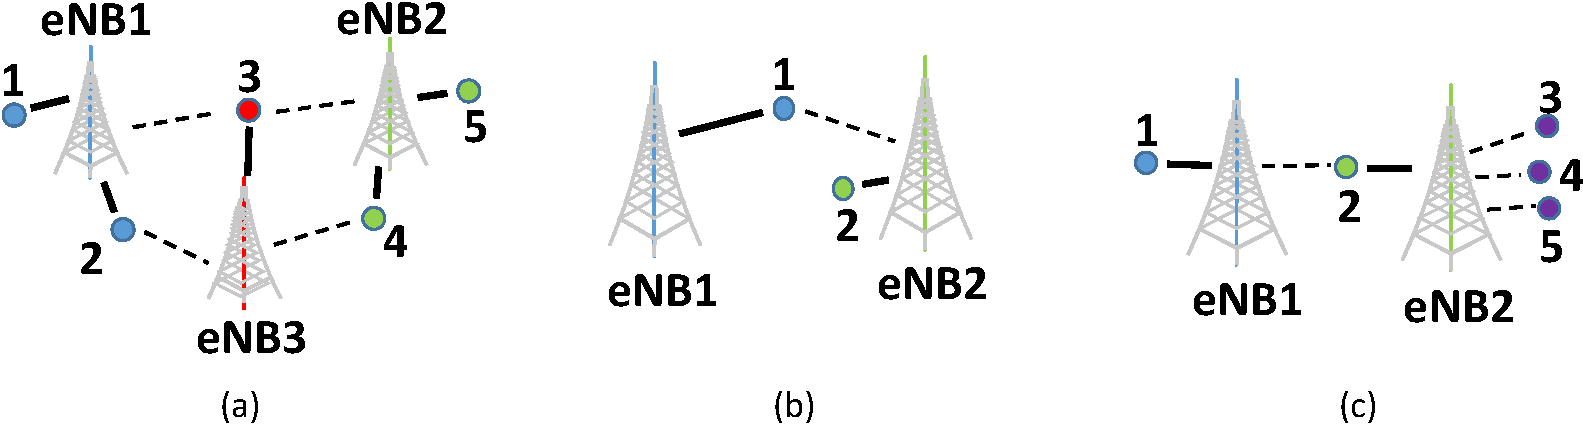
\includegraphics[width=0.9\textwidth, height=0.4\columnwidth]{figs/exampleFigs-crop}
% \caption{Lines reflect associated clients to access points while dashed lines reflect interference. 
%(a) Importance of channel re-use. client 3 can only get its share if access points 1-2 schedule their clients on same two channels. 
%(b) Information asymmetry with two total channels. access point 1 overestimates his share because it cannot sense client 2. (c) Informatrion assymetry with 4 total channels. 
%access point 2 has a share of 1, and while access point 1 can increase his share to 3, 
%it only reserves his fair-share, i.e., 2 channels because it does know how many subchannels 2 is using (1 due to clients 3-5)}
%  \label{fig:asym}
%\end{figure*}




\noindent {\bf Incorrect share:} Figure~\ref{fig:asym}(a) shows an example of incorrect share calculation caused by asymmetric views. 
access point 1 can hear only the PRACH preamble from client 1, whereas eNB2 hears it from both clients 1 and 2. The optimal share for both eNBs is half of the spectrum. 
Because of asymmetry, access point 1 is overestimating its share to be the whole spectrum.

%BR: This is not true. If we don't adjust the share, it will make eNB1 to hop a lot, causing disturbances in the rest of the network...
%This case of information asymmetry is not detrimental to the control plane. It does not affect client 2 because if it did eNB1 would hear it RACH and account for it in the channel allocation. It only affect client1. eNB1 detects this from CQI reports from client1 and adjusts the allocation accordingly and entirely locally. 

This case of information asymmetry is dealt with by the scheduler, \eNB $1$ will sense that there are less free subchannels available than it expected, and will not schedule any transmission in subchannels the client is facing interference on, reducing its effective share. The resulting effective share will still be feasible, allowing the distributed hopping algorithm to converge. However, this share adjustment may not be detected by other neighbors of \eNB $1$, leading to possible inefficiencies.
%in the share calculation algorithm (Figure~\ref{fig:dsc}) 
%through the $\id{free}_{i, j}$ variable. \eNB $1$ will sense that there are less free channels available than it expected, and will update its share. The resulting share will still be feasible, allowing the distributed hopping algorithm to converge. However, this share adjustment may not be detected by other neighbors of \eNB $1$, leading to possible inefficiencies. 

%\begin{figure}[th!]
%  \centering
%    \includegraphics[width=0.45\textwidth]{under}
% \caption{Suboptimal share calculation due to view asymmetry.}
%  \label{underestimation}
%\end{figure}

\noindent {\bf Suboptimal share:} Figure~\ref{fig:asym}(b) shows an example with a total of 4 subchannels, where access point 1 can get one more subchannel since access point 2 can only use one subchannel for its client;
this is because it is interfering with three other clients. Access point 1 limits itself to its estimated share of two subchannels, resulting in under allocation of resources. 
This case of information asymmetry is fundamental of our setup as \eNB $1$ cannot learn about other clients purely from sensing. It can also not be more aggressive in this case as it could unfairly take a share 
from node 2, should the three clients on the right be absent. 

The performance effects of information asymmetries of \cf in general topologies are difficult to analyze precisely. 
In Section~\ref{sec:eval},
 we show that in complex topologies, \cf's performance is comparable to state-of-the-art, centralized resource allocation frameworks for cellular networks~\cite{fermi}.

